\documentclass[12pt]{article}
\usepackage{parskip} % no auto indent
\usepackage{graphicx} % graphics

% My marco file
\usepackage{mymarco}

% Begin page style
\usepackage[margin=1.0in]{geometry}
\usepackage{fancyhdr}
\pagestyle{fancy}
\setlength{\headheight}{15pt}
\rhead{36123040 Shawn Wu} % Define header
\lhead{MATH 321 HW 06} % Put assignment #
\cfoot{\thepage}

\begin{document}

% Problem 1
\begin{fproof}[1(a)]
Let \(\Gamma = \set{\cC(X):\norm{f}\leq 1 \tand N_{\alpha}(f) \leq 1}\).
We appeal to HW5 Problem 3.
We show that \(\Gamma\) is compact by showing that it is closed, bounded, and equicontinous, as \(\Gamma \subseteq \cC(X)\) and \(X\) is compact.

\textbf{Closed:}
We show that \(\Gamma' \subseteq \Gamma\).
Pick any \(g \in \Gamma'\).
There exists a sequence of functions \((g_n) \subseteq \Gamma \setminus \{g\}\) that converges to \(g\) w.r.t. the supremum norm, and this means that \(g_n \to g\) uniformly by Rudin Theorem 7.7.

We show that \(g \in \Gamma\), i.e., \(\norm{g} \leq 1\) and \(N_{\alpha}(g) \leq 1\).

Given any \(\varepsilon > 0\).
We know there exists a natural \(N\) s.t. \(\norm{g - g_N} < \varepsilon\).
Also,
\begin{align*}
    \norm{g} = \norm{g - g_N + g_N} \leq \norm{g-g_N} + \norm{g_N} < 1 + \varepsilon.
\end{align*}
Since \(\varepsilon\) is arbitrary, \(\norm{g} \leq 1\).

Now again given any \(\varepsilon > 0\).
Pick any \(x,y \in X\) where \(x \neq y\).
Then first note that \(d(x,y)>0\) since \(x\neq y\), so \(d(x,y)^{\alpha}\) is a real number greater than zero.
And since \(g_n \to g\) uniformly, there exists a natural \(N\) s.t., \(\abs{g_N(t)-g(t)} < \varepsilon \cdot d(x,y)^{\alpha}/2\), for all \(t \in X\).
Therefore,
\begin{align*}
    \frac{\abs{g(x)-g(y)}}{d(x,y)^{\alpha}} &= \frac{\abs{g(x)-g_N(x) + g_N(y) -g(y) + g_N(x)-g_N(y)}}{d(x,y)^{\alpha}}\\
    & \leq \frac{\abs{g(x)-g_N(x)}}{d(x,y)^{\alpha}} + \frac{\abs{g_N(y)-g(y)}}{d(x,y)^{\alpha}} + \frac{\abs{g_N(x)-g_N(y)}}{d(x,y)^{\alpha}}\\
    &<\frac{\varepsilon \cdot d(x,y)^{\alpha}}{2 d(x,y)^{\alpha}} + \frac{\varepsilon \cdot d(x,y)^{\alpha}}{2 d(x,y)^{\alpha}} + 1\\
    &= 1 + \varepsilon.
\end{align*}
Since \(\varepsilon\) is arbitrary, \(\abs{g(x)-g(y)}/d(x,y)^{\alpha} \leq 1\) for this particular pair of \(x\) and \(y\).
And since \(x,y\) is arbitrary,
then 1 is a upper bound of the set \(A\) where 
\begin{align*}
    A = \set{\frac{\abs{g(x)-g(y)}}{d(x,y)^{\alpha}} : x,y \in X, x\neq y},
\end{align*}
which means that
\begin{align*}
    N_{\alpha}(g) = \sup A \leq 1,
\end{align*}
as the supremum must be the least upper bound.

% Suppose, for the sake of contradiction, \(N_{\alpha}(g) > 1\), i.e., \(N_{\alpha}(g) = 1 + \delta\) for some \(\delta > 0\).
% This means that there exist \(x_0,y_0 \in X, x_0 \neq y_0\) s.t.,
% \begin{align*}
%     \frac{\abs{g(x_0)-g(y_0)}}{d(x_0, y_0)^{\alpha}} > 1 + \delta/2,
% \end{align*}
% as \(1 + \delta/2 < N_{\alpha}(g)\) so \(1 + \delta/2\) is not an upper bound.

% Set \(\lambda = (\delta/2)d(x_0,y_0)^{\alpha}\).
% Note that since \(x_0 \neq y_0\), \(d(x_0, y_0) > 0\).
% Also, as \(\alpha > 0\), \(d(x_0, y_0)^{\alpha} > 0\).
% Thus, \(\lambda > 0\).
% And by rearranging the above inequality,
% \begin{align*}
%     \abs{g(x_0)-g(y_0)} > d(x_0, y_0)^{\alpha} + \lambda.
% \end{align*}
% And since \(g_n \to g\) uniformly, there exists a natural \(N\) s.t. for all \(x \in X\),
% \begin{align*}
%     \abs{g_N(x) - g(x)} < \frac{\lambda}{2}.
% \end{align*}
% This gives in particular that,
% \begin{align*}
%     g(x_0)- \frac{\lambda}{2} < g_N(x_0) < g(x_0) + \frac{\lambda}{2} \text{  and  } g(y_0) - \frac{\lambda}{2} < g_N(y_0) < g(y_0)+ \frac{\lambda}{2}.
% \end{align*}
% This gives that

\textbf{Bounded:}
It's enough to show that \(\Gamma\) can be covered in an open neighborhood in the metric space \((\cC(X), \norm{\cdot})\).
Let \(\opb{0}{2}\) be the open ball centered at the zero function with a radius 2.
We claim that 
\begin{align*}
    \opb{0}{2} \supseteq \Gamma.
\end{align*}
To see this, pick any \(f \in \Gamma\), then \(\norm{f} = \norm{f - 0} \leq 1 < 2\).
Therefore, \(f \in \opb{0}{2}\).

\textbf{Equicontinous:}
Give any \(\varepsilon > 0\).
We aim to find a \(\delta > 0\) s.t.
\begin{align*}
    \abs{f(x)-f(y)} < \varepsilon,
\end{align*}
whenever \(d(x,y) < \delta\), \(x,y \in X\), \(f \in \Gamma\).
We claim that \(\delta = \varepsilon^{1/\alpha}\) will work.
To see this, pick any \(f \in \Gamma\) and any \(x,y \in X\) s.t. \(d(x,y) < \delta\).
Note that either \(x=y\) or \(x\neq y\).
If \(x=y\), then \(\abs{f(x)-f(y)} = 0 < \varepsilon\).
If \(x \neq y\), then
\begin{align*}
    d(x,y) < \delta = \varepsilon^{1/\alpha} \implies d(x,y)^{\alpha} < \varepsilon.
\end{align*}
Also, \(N_{\alpha}(f) \leq 1\) since \(f \in \Gamma\).
This means that
\begin{align*}
    \frac{\abs{f(x)-f(y)}}{d(x,y)^{\alpha}} \leq N_{\alpha}(f) \leq 1 \implies \abs{f(x)-f(y)} \leq d(x,y)^{\alpha} < \varepsilon.
\end{align*}
This proves equicontinuity and concludes the proof of compactness of \(\Gamma\).
\end{fproof}

\begin{fproof}[1(b)]
Let \(\Pi = \set{f \in \cC[0,1]: \norm{f} \leq 1}\).
It's suffice to find a subset \(\Lambda\) of \(\Pi\) that is not equicontinous.
This is due to the fact that if \(\Pi\) is equicontinous, then every subset of \(\Pi\) is as well.

Let \(\Lambda\) be the sequence of functions \(\set{g_n}_{n \in \N}\) where for each \(n\), \(g_n:[0,1] \to \R\) and,
\[
    g_n(x) =
\begin{cases}
    -nx + 1 & \text{ if } 0 \leq x \leq \frac{1}{n},\\
    0 & \text{ otherwise}.
\end{cases}
\]
It's clear that \(\set{g_n} \subseteq \Pi\) since each \(g_n\) is continuous and each \(\norm{g_n} \leq 1\) as \(0 \leq g_n(x) \leq 1\) for all \(n \in \N\) and all \(x \in [0,1]\).

Now let \(\delta_n = 1/n\).
We see that for each \(n\),
\(d(0, 1/(n+1)) = 1/(n+1) < \delta_n\), and
\begin{align*}
    \abs{g_{n+1}(0) - g_{n+1}\pare{\frac{1}{n+1}}} = 1.
\end{align*}
Therefore, we see that there exists an \(\varepsilon = 1 > 0\), s.t. for any \(\delta > 0\),
we can pick two points \(x=0, y=1/(n+1) \in [0,1]\) with \(d(x, y) < \delta_n < \delta\) for some \(n\), and we can pick a function \(g_{n+1} \in \Lambda\) for the same \(n\), s.t. \(\abs{g_{n+1}(x) - g_{n+1}(y)} \geq \varepsilon\).
This proves the negation of the condition for equicontinuity, so \(\Lambda\) is not equicontinous. Hence, the set \(\Pi\) is not equicontinous, which proves it is also not compact by HW5 Problem 3.

\end{fproof}
\newpage

% Problem 2
\begin{fproof}[2]
First note that for any non-constant polynomial \(p\), \(\lim_{x \to \infty} p(x) = +\infty\) if the leading coefficient of \(p\) is positive, and \(\lim_{x \to \infty} p(x) = -\infty\) if the leading coefficient of \(p\) is negative.

Now suppose we have a sequence of polynomials \(p_n \to f\) uniformly on the whole \(\R\).
Then by adopting the Cauchy Criteria, we see that there exists a natural \(N\) s.t. 
\begin{align*}
    \abs{p_N(x) - p_m(x)} < 1,
\end{align*}
for any \(m \geq N\) and \(x \in \R\).
Note that for each \(m \geq N\), \(p_N - p_m\) is also a polynomial, but it doesn't diverge to infinity. This means that \(p_N - p_m\)'s must be constant polynomials, which means that for \(m \geq N\), \(p_m\)'s only differ by constants.

Let \(q\) be the polynomial \(p_N\) without the constant term. Let \(a_0 = \lim_{n \to \infty} p_n(0)\).
We then claim that \(f(x) = q(x) + a_0\), which is a polynomial.
It's suffice to show that \(q(x) + a_0\) is the point-wise limit of the sequence of polynomials \((p_n)\).
Pick any \(t \in \R\).
Consider the sequence of real numbers \((p_n(t))_{n \in \N}\).
Based on previous discussion, we know that for \(n \geq N\), \(p_n\)'s are polynomials that only differ by constant terms.
So, for \(n \geq N\),
\begin{align*}
    p_n(t) = q(t) + p_n(0).
\end{align*}
And we know that \(p_n(0) \to a_0\) as \(n \to \infty\).
Therefore, \(q(t) + p_n(0) \to q(t) + a_0\), which means that \(p_n(t) \to q(t) + a_0\) as \(n \to \infty\).
Hence, \(q(x) + a_0\) is indeed the point-wise limit of \((p_n)_{n \in \N}\).
And since the limit of a sequence real numbers is unique, \(f(x)\) for each \(x\) is therefore a unique real number. This means the limit function \(f\) is unique, which gives that \(f(x) = q(x) + a_0\) and proves that it is a polynomial.

\end{fproof}
\newpage

% Problem 3
\begin{fproof}[3(a)]
Let  \(G = \set{e^{-nx}:n = 0,1,2,3,\cdots}\) be a set of real-valued functions on \([0,1]\).
And let \(\cA\) be an algebra of real-valued continuous functions generated by \(G\), and it's clear that \(\cA\) has the form,
\begin{align*}
    \cA = \set{c_0 + c_1e^{-x}+ c_2e^{-2x} + \cdots + c_ne^{-nx}: n \in \N, c_0, c_1, \cdots, c_k \in \R}.
\end{align*}
To see \(\cA\) is an algebra, pick any \(\alpha \in \R\), \(a=c_0 + c_1e^{-x} + \cdots + c_ne^{-nx}\), \(b=d_0 + d_1e^{-x}+ \cdots + d_me^{-mx} \in \cA\).
Note that we can assume \(n = m\) because if not, say \(n > m\), then we can add on zero terms, i.e., \(d_ie^{-ix}\) where \(d_i = 0\), to the end of \(b\).
Therefore,
\begin{align*}
    a+b = (c_0 + d_0) + (c_1+d_1)e^{-x} + (c_2+d_2)e^{-2x} + \cdots + (c_n + d_n)e^{-nx} \in \cA.
\end{align*}
And,
\begin{align*}
    a \cdot b = c_0d_0 + (c_0d_1 + c_1d_0)e^{-x} + \cdots + \pare{\sum_{i+j = n+m}c_id_j}e^{-(n+m)x} \in \cA.
\end{align*}
Lastly,
\begin{align*}
    \alpha b = \alpha d_0 + \alpha d_1 e^{-x} + \cdots + \alpha d_m e^{-mx} \in \cA.
\end{align*}
So, \(\cA\) is closed under addition, multiplication, and scalar multiplication, which makes \(\cA\) an algebra.

Also note that on \([0,1]\), \(e^{-nx}\) is strictly monotone decreasing for \(n \geq 1\), which makes \(\cA\) separate points. And on \([0,1]\), \(e^{-nx}\) is strictly positive for \(n \geq 0\), which makes \(\cA\) vanishes at no points.
Therefore, by Stone-Weistrass Theorem, the uniform closure of \(\cA\) is \(\cC([0,1])\).

Now pick any continuous real-valued function \(f\) on \([0,1]\).
Based on our discussion before, there exists a sequence of functions \((\varphi_n) \subseteq \cA\) s.t. \(\varphi_n \to f\) uniformly.
Note that since each \(\varphi_n\) is of the form 
\begin{align*}
    c_0e^{-0x} + c_1e^{-x} + \cdots + c_ke^{-kx},
\end{align*}
by the linearity of Stieltjes integrals,
\begin{align*}
    \int_{0}^{1} \varphi_n \dalf &= c_0\int_{0}^{1} e^{-0x} \dalf + c_1 \int_{0}^{1} e^{-x} \dalf + \cdots + c_k \int_{0}^{1}e^{-kx} \dalf, \text{ and }\\
    \int_{0}^{1} \varphi_n \dbet & = c_0\int_{0}^{1} e^{-0x} \dbet + c_1 \int_{0}^{1} e^{-x} \dbet + \cdots + c_k \int_{0}^{1}e^{-kx} \dbet.
\end{align*}
And since \(\int_{0}^{1} e^{-mx} \dalf = \int_{0}^{1} e^{-mx} \dbet\) for each \(m = 0, 1, 2, \cdots,\) \(\int_{0}^{1} \varphi_n \dalf = \int_{0}^{1} \varphi_n \dbet\) for each \(n \in \N\).
Therefore, \((\int_{0}^{1}\varphi_n \dalf)_{n \in \N}\) and \((\int_{0}^{1} \varphi_n \dbet)_{n \in \N}\) are the same sequence of real numbers, and hence their limits are the same, if they exist.

Also, since \(\varphi_n \to f\) uniformly on \([0,1]\), by Rudin Theorem 7.16,
\begin{align*}
    \int_{0}^{1} f \dalf &= \lim_{n \to \infty} \int_{0}^{1} \varphi_n \dalf, \text{ and similarly,}\\
    \int_{0}^{1} f \dbet &= \lim_{n \to \infty} \int_{0}^{1} \varphi_n \dbet.
\end{align*}
And since the two limits are the same,
\begin{align*}
    \int_{0}^{1} f \dalf = \int_{0}^{1} f \dbet,
\end{align*}
as desired.
\end{fproof}

\begin{fproof}[3(b)]
The claim is true and we give a direct proof.
First note that \(\alpha(x) = \beta(x)\) when \(x = 0\) since they are both zero when \(x =0\).

Also, since \(e^{-0x} = 1\) for any \(x \in [0,1]\),
\begin{align*}
    \int_{0}^{1} e^{-0x} \dalf &= \int_{0}^{1} \dalf = \alpha(1) - \alpha(0) = \alpha(1), \text{ and similarly,}\\
    \int_{0}^{1} e^{-0x} \dbet & = \beta(1).
\end{align*}
Since \(\int_{0}^{1} e^{-0x} \dalf = \int_{0}^{1} e^{-0x} \dbet\), \(\alpha(x) = \beta(x)\) when \(x = 1\).

Now for any \(x \in (0,1)\).
We first construct a sequence of functions \((f_n(t))\) on \([0,1]\) that approaches point-wise to the heavy-side step function on \([0,1]\), \(H_x(t)\) where,
\[
H_x(t) = 
\begin{cases}
    1, & t \in [0,x]\\
    0, & t \in (x,1].
\end{cases}
\]
First let \(\varepsilon_n = (1-x)/2^n\).
It's clear that \(\varepsilon_n \to 0\), each \(\varepsilon_n\) is nonzero,  and \(x + \varepsilon_n \in (x,1)\).
Now for each \(n\), define 
\[
f_n(t) = 
\begin{cases}
    1, & t \in [0,x]\\
    -\frac{1}{\varepsilon_n} t + \frac{x + \varepsilon_n}{\varepsilon_n}, & t \in (x, x + \varepsilon_n),\\
    0, & t\in [x + \varepsilon_n, 1].
\end{cases}
\]
\begin{center}
    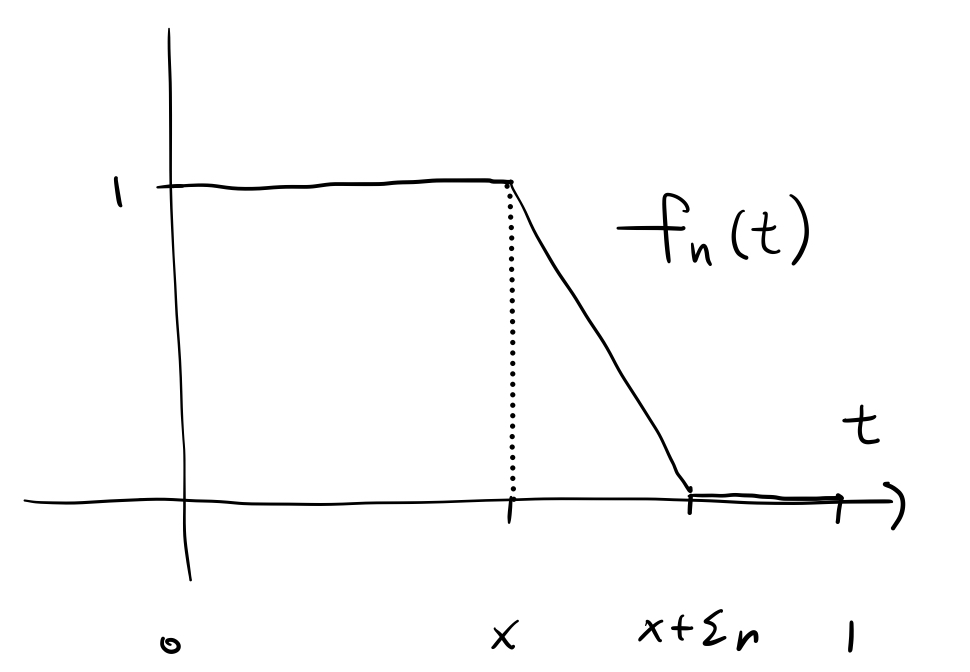
\includegraphics[scale=0.2]{Asst6.3b.jpeg}
\end{center}
Therefore, for each \(n\),
\begin{align*}
    \int_{0}^{1}f_n(t) \dalf(t) = \int_{0}^{x} f_n(t) \dalf(t) + \int_{x}^{x+\varepsilon_n} f_n(t) \dalf(t) + \int_{x+\varepsilon_n}^{1} f_n(t) \dalf(t).
\end{align*}
Note first that \(\int_{0}^{x} f_n(t) \dalf(t) = \alpha(x)\) and \(\int_{x+\varepsilon_n}^{1} f_n(t) \dalf(t) = 0\).
Also,
\begin{align*}
    \int_{x}^{x+\varepsilon_n} f_n(t) \dalf(t) \leq \int_{x}^{x+\varepsilon_n} 1 \dalf(t) = \alpha(x + \varepsilon_n) - \alpha(x).
\end{align*}
Therefore, combining the above equalities/inequalities,
\begin{align*}
    \int_{0}^{1} f_n(t) \dalf(t) \leq \alpha(x) + \alpha(x + \varepsilon_n) - \alpha(x) + 0 = \alpha(x+\varepsilon_n).
\end{align*}
Also, since \(f_n(t) \geq 0\) on \([x, x+ \varepsilon_n]\), therefore \(\int_{x}^{x+\varepsilon_n} f_n(t) \dalf(t) \geq 0\).
This gives that
\begin{align*}
    \alpha(x) = \int_{0}^{x} f_n(t) \dalf(t) \leq \int_{0}^{1} f_n(t) \dalf(t).
\end{align*}
Combining the above results, we have
\begin{align*}
    \alpha(x) \leq \int_{0}^{1} f_n(t) \dalf(t) \leq \alpha(x + \varepsilon_n).
\end{align*}
Since \(\alpha\) is continuous, as \(\varepsilon_n \to 0\), \(x + \varepsilon_n \to x\), so \(\alpha(x + \varepsilon_n) \to \alpha(x)\).
Therefore, \(\int_{0}^{1} f_n(t) \dalf(t) \to \alpha(x)\) by Squeeze Theorem.
And by a similar reasoning, \(\int_{0}^{1} f_n(t) \dbet(t) \to \beta(x)\).

Note that since each \(f_n\) is continuous, by the results of (a), \((\int_{0}^{1} f_n(t) \dalf)\) and \((\int_{0}^{1} f_n(t) \dbet)\) are essentially the same sequence of real numbers.
Since the limit of a sequence of real numbers is unique, \(\alpha(x) = \beta(x)\).
This concludes the proof that \(\alpha(x) = \beta(x)\) on the whole \([0,1]\).
\end{fproof}
\newpage

% Problem 4
\begin{fproof}[4]
Note that the algebra \(\cA\) in question either vanishes at no points in \(K\) or it vanishes at some points in \(K\). If it's the former, then by Stone-Weistrass Theorem, \(\overline{\cA}\) consists of all continuous real-valued functions on \(K\); this is case (i). If, however, \(\cA\) does vanish at some point in \(K\), say \(p \in K\). Let \(\cF\) by the set of all continuous functions on \(K\) that vanish at \(p\). For case (ii), it remains to show that \(\overline{\cA} = \cF\).

Pick any \(f \in \overline{\cA}\).
This means that there exists a sequence of functions \((f_n) \subseteq \cA\) that converges uniformly to \(f\).
This means that \(f\) is the limit function of \(f_n\), i.e.,
\begin{align*}
    f(p) = \lim_{n \to \infty} f_n(p) = \lim_{n \to \infty} 0 = 0.
\end{align*}
Therefore, \(f \in \cF\).
This shows that \(\overline{\cA} \subseteq \cF\).

Now pick any \(f \in \cF\).

First note that \(\cA + \R\) is an algebra of continuous real-valued functions that both separate points and vanishes at no points.
To see \(\cA + \R\) separate points, note that \(\cA\) separate points and \(\cA = \cA + 0 \subseteq \cA + \R\). 
To see \(\cA + \R\) vanishes at no points, pick any \(x \in K\). Then either \(\cA\) vanishes at \(x\) or not.
If \(\cA\) doesn't not, then \(\cA + \R\) being a superset of clearly also doesn't not vanish at \(x\); if it does, then there exists \(\alpha \in \cA\) s.t. \(\alpha(x) = 0\), so \(\alpha(x) + 1 \neq 0\) where \(\alpha(x) + 1 \in \cA + \R\), which means that \(\cA + \R\) doesn't not vanish at \(x\), and hence it vanishes at no points in \(K\) at \(x\) is an arbitrary point in \(K\).

Lastly, to see \(\cA\) is an algebra, pick any \(\varphi + a, \psi + b \in \cA + \R\) where \(a,b \in \R\) and \(c \in \R\).
Note that
\begin{align*}
    \varphi + a + \psi + b = (\varphi + \psi) + (a + b) \in \cA + \R,
\end{align*}
as \(\varphi + \psi \in \cA\), \(a+b \in \R\), since both \(\cA\) and \(\R\) are closed under addition.
Also,
\begin{align*}
    (\varphi + a)(\psi + b) = (\varphi \psi + a \psi + b \varphi) + ab \in \cA + \R,
\end{align*}
as \(\varphi \psi + a \psi + b \varphi \in \cA\) and \(ab \in \R\). It's clear that \(ab \in \R\) as \(\R\) is closed under multiplication. To see \(\varphi \psi + a \psi + b \varphi \in \cA\), note that \(\varphi \psi \in \cA\) since \(\cA\) is closed under multiplication, \(a \psi, b \varphi \in \cA\) since \(\cA\) is also closed under scalar multiplication, so the sum of the three is in \(\cA\) since \(\cA\) is closed under addition.
Also, it clearly that
\begin{align*}
    c(\varphi + a) = c \varphi + ca \in \cA + \R,
\end{align*}
as both \(\cA\) and \(\R\) are closed under scalar multiplication.

Therefore, by Stone-Weistrass Theorem, \(\overline{\cA + \R} = \cC(K)\). This means that there exists a sequence of functions \((f_n + c_n) \subseteq \cA + \R\), where \((f_n) \subseteq \cA\) and \((c_n) \subseteq \R\), that approaches uniformly to the function \(f\) in \(\cF\) we have picked before.

It remains to show that \(f_n \to f\) uniformly on \(K\), which gives \(\cF \subseteq \overline{\cA}\).
Given any \(\varepsilon > 0\).
Since \(f_n + c_n \to f\) uniformly on \(K\), there exists a natural \(N\) such that for \(n > N\),
\begin{align*}
    \abs{(f_n(x) + c_n) - f(x)} < \frac{\varepsilon}{2},
\end{align*}
for any \(x \in K\).
In particular,
\begin{align*}
    \abs{(f_n(p) + c_n) - f(p)} < \frac{\varepsilon}{2}, \text{ or simply } \abs{c_n} < \frac{\varepsilon}{2},
\end{align*}
since \(f\) and all \(f_n\) vanish at the point \(p\).
Now note that for any \(n > N\),
\begin{align*}
    \abs{f_n(x) - f(x)} = \abs{(f_n(x) + c_n - f(x)) - c_n} \leq \abs{f_n(x) + c_n - f(x)} + \abs{c_n} < \frac{\varepsilon}{2} + \frac{\varepsilon}{2} = \varepsilon,
\end{align*}
for any \(x \in K\).
This concludes the step that \(f_n \to f\) uniformly on \(K\), which concludes the entire proof.
\end{fproof}
\newpage

% Problem 5
\begin{fproof}[5]

\end{fproof}
\end{document}